%% 
%% Copyright 2007-2020 Elsevier Ltd
%% 
%% This file is part of the 'Elsarticle Bundle'.
%% ---------------------------------------------
%% 
%% It may be distributed under the conditions of the LaTeX Project Public
%% License, either version 1.2 of this license or (at your option) any
%% later version.  The latest version of this license is in
%%    http://www.latex-project.org/lppl.txt
%% and version 1.2 or later is part of all distributions of LaTeX
%% version 1999/12/01 or later.
%% 
%% The list of all files belonging to the 'Elsarticle Bundle' is
%% given in the file `manifest.txt'.
%% 
%% Template article for Elsevier's document class `elsarticle'
%% with harvard style bibliographic references

\documentclass[preprint,12pt]{elsarticle}

%% Use the option review to obtain double line spacing
%% \documentclass[preprint,review,12pt]{elsarticle}

%% Use the options 1p,twocolumn; 3p; 3p,twocolumn; 5p; or 5p,twocolumn
%% for a journal layout:
%% \documentclass[final,1p,times]{elsarticle}
%% \documentclass[final,1p,times,twocolumn]{elsarticle}
%% \documentclass[final,3p,times]{elsarticle}
%% \documentclass[final,3p,times,twocolumn]{elsarticle}
%% \documentclass[final,5p,times]{elsarticle}
%% \documentclass[final,5p,times,twocolumn]{elsarticle}

%% For including figures, graphicx.sty has been loaded in
%% elsarticle.cls. If you prefer to use the old commands
%% please give \usepackage{epsfig}

%% The amssymb package provides various useful mathematical symbols
\usepackage{amssymb}

\usepackage{amsmath}

\usepackage{amsfonts}
\usepackage{graphicx}
\newcommand{\Rho}{\mathrm{\textit{P}}}
\usepackage{subcaption}
\usepackage{csquotes}
\usepackage{algorithm} 
\usepackage{algpseudocode} 
\usepackage{longtable}
%\usepackage[top=1.0in, bottom=1.0in, left=1.0in, right=1.0in]{geometry}
\usepackage{url}
\def\UrlBreaks{\do\/\do-}
\usepackage{breakurl}
\usepackage[breaklinks]{hyperref}
%% The amsthm package provides extended theorem environments
%% \usepackage{amsthm}

%% The lineno packages adds line numbers. Start line numbering with
%% \begin{linenumbers}, end it with \end{linenumbers}. Or switch it on
%% for the whole article with \linenumbers.
%% \usepackage{lineno}

\journal{Information Sciences}

\begin{document}

\begin{frontmatter}

%% Title, authors and addresses

%% use the tnoteref command within \title for footnotes;
%% use the tnotetext command for theassociated footnote;
%% use the fnref command within \author or \address for footnotes;
%% use the fntext command for theassociated footnote;
%% use the corref command within \author for corresponding author footnotes;
%% use the cortext command for theassociated footnote;
%% use the ead command for the email address,
%% and the form \ead[url] for the home page:
%% \title{Title\tnoteref{label1}}
%% \tnotetext[label1]{}
%% \author{Name\corref{cor1}\fnref{label2}}
%% \ead{email address}
%% \ead[url]{home page}
%% \fntext[label2]{}
%% \cortext[cor1]{}
%% \affiliation{organization={},
%%             addressline={},
%%             city={},
%%             postcode={},
%%             state={},
%%             country={}}
%% \fntext[label3]{}

\title{A Ranked Solution for Social Media Fact Checking Using Epidemic Spread}

%% use optional labels to link authors explicitly to addresses:
%% \author[label1,label2]{}
%% \affiliation[label1]{organization={},
%%             addressline={},
%%             city={},
%%             postcode={},
%%             state={},
%%             country={}}
%%
%% \affiliation[label2]{organization={},
%%             addressline={},
%%             city={},
%%             postcode={},
%%             state={},
%%             country={}}

\author[inst1]{John Hawthorne Smith}

%\affiliation[inst1]
%        {organization={Northwestern University},
%        addressline={633 Clark St},
%        city={Evanston}, postcode={60208},
%        state={IL},
%        country={United States}}

\author[inst2]{Author Two}

\begin{abstract}
%% Text of abstract
Within the past decade, social media has become a primary platform for consumption of information and current events. Unlike with traditional news sources, however, social media posts do not have to go through a rigorous validation process prior to publication. The 2019 Mueller Report illustrates how malicious actors have taken advantage of these lax requirements to sway public opinion on topics from the \#blacklivesmatter movement to the 2016 U.S. Presidential election. 

Currently, social media companies rely primarily on communal-policing of misinformation: this is unlikely that this will happen with regularity. To counteract this, other literature on the topic is focused on building neural networks that will be able to detect accurate from misleading content; however, the rapidly evolving nature of misinformation means that they will have to be retrained and redeployed on an iterative and time-consuming basis.

This article, therefore, proposes a novel approach to the problem: treating misinformation as a virus. This article proposes a ranking system that third-party fact checkers can utilize to prioritize posts for checking. This algorithm is then tested against multiple data sets with strong positive results, decreasing viral spread in a matter of minutes.
\end{abstract}


\begin{keyword}
%% keywords here, in the form: keyword \sep keyword
Social media \sep Fake news \sep Misinformation \sep Partisanship \sep Networks
\end{keyword}

\end{frontmatter}

%% \linenumbers

%% main text
\section{Introduction}
\label{Introduction}

%% For citations use: 
%%       \citet{<label>} ==> Jones et al. [21]
%%       \citep{<label>} ==> [21]
%%

In 2018, social media overtook print media as the fourth most popular source of news for Americans. As of 2019, 20\% ``often" got their news from social media \cite{shearer2018social}, while 68\% of all American got their news from social media at least occasionally \cite{matsa2018news}. This is not inherently a bad thing - in countries with authoritarian leaders and state-run media, social media may be the only outlet for opposition spokespeople to share their messages \cite{walker2014breaking}; ordinary citizens can now contribute their stories and experiences without the high financial barrier to entry that traditional journalism requires \cite{qualman2012socialnomics, tapscott2008wikinomics}; in unmanageable situations and crises, such as the 2017 Manchester bombing, social media allows for the instantaneous exchange of information between individuals and emergency management agencies \cite{mirbabaie2020breaking, eriksson2016facebook}; in situations like the COVID-19 pandemic, where information is rapidly evolving, social media allows for immediate knowledge dissemination by dramatically shortening the traditional time from publication to widespread translation to adoption \cite{chan2020social}. 
 
However, not all information shared on social media is true, and the subset of people who primarily get their news from social media tend to be less engaged, less knowledgeable of current events, more likely to hear unproven claims and conspiracy theories than those who get their news from more traditional sources, and are more likely to believe these conspiracies \cite{mitchell2020americans}. In just two examples of this, Edgar Maddison Welch drove from North Carolina to Washington D.C. with an AR-15 to investigate a fake pedophile conspiracy ring known as ``pizzagate" in December 2016, \cite{goldman2016comet}; in 2018, Burmese officials created over 1,000 Facebook posts filled with hate speech and detailing fake crimes committed by the Rohynga Muslim minority to justify one of the largest forced migrations in recent history \cite{subedar2018country}.

Exacerbating this problem, the spread of correct information is much slower than that of misinformation: while true rumors tend to be validated within 2 hours of the first tweet, false rumors take about 14 hours to be debunked \cite{zubiaga2016analysing,shao2016hoaxy}. This is a problem since, in a crisis event, 50\% of all retweets occur within the first hour after a tweet is shared and 75\% are within the first day \cite{kwak2010twitter}. Even if an untrue story is debunked, corrective information does not reach as broad of an audience as misinformation does \cite{maddock2015characterizing, vosoughi2018spread}, and, in some cases, rumors and other fake stories actually see an increase in spread \textbf{after} they have been debunked \cite{starbird2014rumors}. In fact, this fits a pattern where highly controversial and politicized topics spark backfire effects when passionately held misconceptions are challenged \cite{gollust2009polarizing,nyhan2010corrections,nyhan2013hazards,redlawsk2010affective,schaffner2016misinformation,hart2012boomerang}.

Therefore, an alternative solution is necessary that can stop the rapid spread of misinformation in a timely fashion. 

\section{Literature Review}
Social media companies such as Facebook and Twitter currently have policies to prevent the spread of misinformation, but they are severely limited. Mark Zuckerberg, the CEO of Facebook, has spoken at length that a superior solution is needed to what is currently implemented \citep{energy2018facebook,zuckerberg2020}. Facebook requires a post to be reported before it can be fact-checked \citep{owen2016clamping}, and a CNN attempts to prevent further posts of the same content (such as re-sharing an image) \citep{carion2020end}, however these two steps are easily outwitted by malicious actors \citep{sumbaly2020using,dean2020facebook,Fung2020facebook}. Twitter currently only allows for flagging of political misinformation that is directly related to a political event, census, or impersonation \citep{twitter2021rules}, and their misinformation approach is primarily crowd-sourced \cite{birdwatch2021twitter}, which has a high margin for error without a clear person in charge \cite{hara2016co}.

The current proposed solutions from published journal articles generally fall into two groupings: tools that seek to recognize all misinformation and tools that seek to recognize particular subsets of misinformation (i.e. spam).

Language analysis is, clearly, a broad subject of analysis.  Castillo et al. use a decision tree based off emojis, symbols, etc. to attempt to predict misinformation \cite{castillo2011information}. Other textual analysis includes Qazvinian's analysis of speech tags \cite{qazvinian2011rumor}, Takahashi \& Igata's examination of ``clue" words \cite{takahashi2012rumor}, Gupta et al.'s exploration of the usage of profanity \cite{gupta2014tweetcred}, Ghosh, Guo, and Muresan's investigation of word embeddings \cite{ghosh2015sarcastic}, Potomias, Siloas, and Stafylopatis's usage of a transformer \cite{potamias2020transformer}, Gaucho et al.'s review of tensor embeddings to detect content \cite{guacho2018semi}, Rubin et al.'s \cite{rubin2016fake} and Horne and Adali's \cite{horne2017just} usage of linguistic SVM classifications, Popat's investigation of how assertive verbs are in true vs. untrue content \cite{popat2017assessing}, and Riloff's \cite{riloff2013sarcasm}, Pt{\'a}{\v{c}}ek et al.'s \cite{ptavcek2014sarcasm}, Buschmeier's \cite{buschmeier2014impact}, and Barbieri's \cite{barbieri2014modelling} attempt to identify sarcasm.

For the tools that seek to recognize \textbf{all} misinformation, the most common solution is an RNN or an RNN/CNN combination. Ma et al. use a CNN to detect unique language patterns \cite{ma2018rumor} and Xu et al. use an RNN for the same purposes \cite{xu2019deep}, while Liu and Wu \cite{liu2018early}, Yang et al. \cite{yang2012automatic}, Wang et al. \cite{wang2018eann} Shu et al. \cite{shu2019role}, and Lee and Dernoncourt \cite{lee2016sequential}, Shu et al. \cite{shu2019beyond,shu2020leveraging} propose combination RNN/CNN solutions based off of text as well as user features (e.g. registration age) or visual clues to determine likely fake posts.  Other machine learning solutions also work off a combination of text and user information \cite{sun2013detecting,kwon2017rumor,ma2015detect,ma2016detecting,zhao2015enquiring}. VanDam uses a combination of a supervised and supervised neural network to detect hashtag and account hijacking \cite{vandam2019learning}. Chen proposes an improvement to the RNN solutions by using an attention based RNN \cite{chen2018call}. Khoo et al. also use an attention based transformer and include a hierarchical token and post level model as well \cite{khoo2020interpretable}. Zhou's SAFE model is CNN only, but it attempts to cover the same ground in a similar fashion \cite{zhou2020mathsf}.

In terms of graph analysis, Wu, Yang, and Zhu \cite{wu2015false} use a graph-kernel SVM to classify misinformation as does Ma at al. \cite{ma2017detect}. Jin et al. \cite{jin2013epidemiological} and Wu et al. \cite{wu2016mining} both identify that this problem is naturally suited to epidemiological spread. Ren et al. use a Graph Neural Network (GNN) to classify news sharing nodes \cite{ren2020adversarial} -- a similar goal to other works that focus on the user sharing the content. Hamid et al. use a GNN with a Bag of Words and BERT model \cite{hamid2020fake}, Han et al. use a GNN with continual learning \cite{han2020graph}, Rath, Morales, and Srivastava use an attention based GNN \cite{rath2021scarlet}, while Benimara et al. use a combination of semi-supervised learning and a GNN to solve the problem \cite{benamira2019semi}. Gupta et al. use a graph optimization approach \cite{gupta2012evaluating}, while others use a propagation model which tracks the cascade of content \cite{jin2016news,jin2014news,zhou2018fake,kashima2003marginalized}. Huang et al. use a combination of a GNN and a propagation model \cite{huang2019deep}. Ciampaglia et al. \cite{ciampaglia2015computational} and Shi and Weninger \cite{shi2016discriminative} use knowledge graphs and subject-predicate-object triples. Mishra et al. have used GNN's for abuse detection \cite{mishra2019abusive}, Li and Goldwasser \cite{li2019encoding} and del Tredici et al. \cite{del2019you} for political partisanship detection. Han et al. \cite{han2020graph}, Nguyen et al. \cite{nguyen2020fang}, and Chandra et al. \cite{chandra2020graph} have applied GNNs recently to the topic of fake news detection. 
 
\subsection{Reasons for Alternative Solution}
There are two primary reasons why these previously discussed solutions are ineffective: scale and content.

\subsubsection{Scale}
The issue of scale is not only non-trivial, but is unmentioned in the other literature on solving this issue. Attempting to crawl through every tweet and every URL posted would be an incredibly difficult task given that Facebook alone has 1.8 \textbf{billion} daily active users according to their Q3 2020 earnings report, with 2.54 billion daily active users of at least one tool in the Facebook portfolio (Facebook, Instagram, WhatsApp, etc.) --  those numbers balloon to 2.74 and 3.21 billion on a monthly level \cite{facebook2020q3}. Given that in 2014 Facebook generated 4 petabytes of data daily and ran 600,000 queries with 1 million map-reducing jobs when their total daily active users was 890 million \cite{bronson2015open}, a simple ratio would provide a conservative estimate that Facebook now generates at least 8.1 petabytes of data every day, with 1.2 million queries and 2.1 million map-reducing jobs. 

Many of the proposed solutions for fake news detection are RNN based, however RNNs are far too resource heavy to be successfully implemented at the necessary scale \cite{gehring2017novel, sze2017efficient}. Even transformer based attention models require high amounts of computational power and primarily excel at tasks like language translation \cite{vaswani2017attention}. 

The GNNs mentioned in the literature review section similarly struggle with scale. Han et al.'s GNN, for example, only looks at surface level user data such as length of user name; Chandra et al.'s GNN looks at who is consistently sharing misinformation, but it is topic specific as well and requires an extensive history of historical misinformation sharing; Nguyen et al's GNN creates only two homogeneous graphs - one looking at news sources and one looking at users - which misses the clear connections between the patient zeroes and the spread of a disease.

Every single neural network discussed here is therefore ``hack-able" at the point that malicious actors determine the pattern being used to allocate a post into a remove/don't-remove bucket. Several of these neural networks include surface level data like length of user name -- if a malicious actor discovers that their disinformation is being flagged simply based off of user name length, all they have to do is change their user name and their content is allowed to flow freely. This would require every one of these neural networks to be re-trained on an iterative basis, which is unsustainable.

\subsubsection{Content}
There are two primary content issues. First, as Liu points out in their 2019 thesis \cite{liu2019early}, each RNN is topic specific. Because of that, it begins with 0 information when the misinformation topic begins and requires a great deal of time to build up enough of a base to be successfully trained and deployed. In some crisis situations, that time may not be available. This criticism holds true for the propagation models as they require too much time before they can be successfully deployed.

Second, current literature using NLP to decipher sarcasm and irony primarily revolves around unexpected word combinations \cite{barbieri2014modelling,buschmeier2014impact,ghosh2015sarcastic} or RoBERTa recurrent neural networks \cite{potamias2020transformer}. Many of these are able to generate quite high F1 scores; however, as Oprea and Magdy point out, tools that are successful in one data set struggle in other data sets. Models trained in the Riloff data set can generate an F1 score above 0.8, but those same models will generate an F1 score near 0.5 (which is the same as random guessing) when applied to the Pt{\'a}{\v{c}}ek set \cite{oprea2019exploring}. This implies there are extreme differences in how groups express and perceive irony/sarcasm/hyperbole. Those differences are beyond the scope of what RNNs and RCNNs can currently successfully grasp.

An acceptable solution must be able to handle constantly shifting content topics without needing to be retrained on a daily basis, and it cannot incorrectly flag sarcastic content as ``false".

\section{Methodology}
\label{methodology}
Instead, this work proposes that misinformation be treated as a virus, where fact-checking is akin to vaccination. The current solution works as a de-facto uniform vaccination -- in order for that solution to work, upwards of 80\% of all posts would have to be fact-checked \cite{may1984spatial,hethcote2014gonorrhea,hethcote2013modeling,hethcote1987epidemiological,albert2000error, pastor2001epidemic}, as a network can remain contagious even after the majority of nodes are removed \cite{cohen2000resilience}. Indeed, in this context, the fraction of content $v_c$ that would need to be fact-checked/vaccinated and removed in order to make the network no longer contagious, $v_c \rightarrow 1$ \cite{cohen2003efficient,strogatz2001exploring,albert2002statistical,dorogovtsev2002evolution,pastor2002immunization}. 

An alternative solution may be a proportional fact-check, where the fraction of posts to be fact checked is proportional to their relevance in the network. While this is more effective than uniform immunization, it is not the most efficient solution \cite{dezsHo2002halting,anderson1992infectious}. The fraction needed to vaccinate, $v_c \approx \lambda^2/3 $, where $\lambda$ is the rate of spread of a disease \cite{pastor2002immunization,barabasi1999emergence}. This is better than $v_c \rightarrow 1$, but not ideal. Networks are incredibly resistant to the loss of random nodes and are able to recover quickly, but dissolve quickly when a small properly targeted fraction of nodes are removed  \cite{albert2000error,callaway2000network,cohen2003efficient,helleringer2007sexual,cohen2001breakdown,hethcote2014gonorrhea,cohen2000resilience}.

Therefore, for a set of tweets, $ t \in T$, that must be fact-checked, $F \subset T$, we can create an ordered set $F^*$ such that $F^* = (t^*, t_1, t_2 \cdots t_n), \ t^* \succ t_1 \succ t_2 \cdots \succ t_n$. To determine the ranking, let $\mu \in \mathcal{M} | \mathcal{M} \in \mathbb{R}$ be the set of relevant numerical metrics available for each user/tweet combination and $\beta \in B| B \in \mathbb{R}$ be the set of unique weights per metric. These can be summed: $\zeta = \sum_{n=0}^{|\mathcal{M}|} \beta_{n} \cdot \mu_{n}$, meaning for tweets $t_i$ and $t_j$: $\zeta_i > \zeta_j \Rightarrow t_i \succ t_j | t_i, t_j \in F$.
 
This allows for the fact that there will always be more posts that need to be checked than can be physically checked in a day, but also ensures that the most dangerous -- the ``super-spreaders" -- are stopped first.

\subsection{$\mu_1$: User Importance}
\label{mu1}
Typically in network theory, $k$ represents the number of connections a nodes has, but it is directionally agnostic. Since directionality is important is social media ($i$ follows $j$ does not imply $j$ follows $i$), let $\psi$ represent a ``following" connection, such that $\psi_{ij}$ represents user $i$ following user $j$. 

Because social media seeks to connect like minded individuals, it has a tendency to generate \textit{echo-chambers}, or closed networks with high repetition of content and low diversity of thought \cite{adibi2005proceedings, bastian2009international, pariser2011filter,bozdag2015breaking}. This means that $\rho_k$, the partisan leaning of some unique user, $u_k$, is directly proportional to the average partisan leaning of the \textit{echo-chamber} network $n_n$: $\rho_k \sim \langle \rho_n \rangle$ \cite{asch1956studies,bullock2007experiments}, which allows for malicious actors to push the average partisanship of the network, $\langle \rho_n \rangle$, to extremes \cite{shin2018diffusion,bastos2019brexit,hegelich2016social,mueller2019mueller}. By factoring in the Barab{\'a}si-Albert preferential equation, this equation becomes: $\langle \rho_n \rangle = \sum_{i=1}^{|n_n|}\rho_i\psi_i / \sum_{j}\psi_j, (u_i \in n_n, n_n \in N)$. This equation effectively operates as a weighted average based off of the number of inbound connections. However, while a user with a high $\psi$ value may have an outsized voice in one network, they will not necessarily in another -- highly conservative content will not be nearly as persuasive to a liberal audience as a conservative one. Therefore, let $\iota$ represent an adapted version of the Hopfield attractor network \cite{hopfield1982neural,hopfield1985neural,nowak1998toward,kitts1999structural,macy2003polarization} function that calculates the likelihood that a user will be immune to a particular strain of misinformation, where $\rho_{\Delta}$ is the absolute value of the difference between the partisanship of the user, $i$, and the content provider, $c$: $\iota(\rho_{\Delta})=1 / (1+\exp{\big(-10 (\rho_{\Delta_{ic}}-0.5)\big)})$. This can then be used to calculate $\langle \tilde{\psi} \rangle =  \psi P(\psi)(1-\iota)$. $\tilde{\psi}$ more accurately represents connections than $k$ or $\psi$ as it more thoroughly matches the S-I-R model where nodes are categorized as susceptible–infected–removed \cite{ferrari2006network,bailey1975mathematical,newman2005threshold,newman2002spread}. In this model, it is standard to remove immune nodes from the network as they will neither transmit nor be infected by the disease; here, people highly opposed to a certain content are unlikely to be persuaded or further share it. 

Let $\vec{A_i}$ be a vector of ordered pairs of all users that $u_i$ follows and their corresponding follower counts:
$\vec{A_i}=\{(u_1,|\tilde{\psi}_1|),\dots (u_n,|\tilde{\psi}_n|)\}, \psi \in \Psi$. The most important user in this vector is the user with corresponding $\max(|\tilde{\psi}|)$. This allows for private groups, reportedly a key place where the riot at the U.S. Capitol on January 6th was planned and misinformation was spread \cite{yin2021facebook,horwitz2020facebook}, to be included: the most important person in the group is the person with  $\max|\psi|$ for said group; similarly, the group can be included in $\vec{A_i}$ for the user, where the corresponding $\psi$ value is the number of members who belong to it. Let $U^*$ then be the set of all users who are a $u^*$ for at least one other user. We can then determine the number of times a particular user appears in that set, which will be the first metric: 
\begin{equation}
\label{mu_1 equation}
    \mu_1 = \sum_{u\ \in \ U^*}1_{\{u_i\}}(u)
\end{equation}

This proposed equation operates as a more refined version of Cohen et al.'s strategy for immunization \cite{cohen2003efficient}, which has been proven to be effective with ecological networks \cite{sole2001complexity,camacho2002robust}, metabolic networks \cite{jeong2000large}, cellular proteins \cite{jeong2001lethality}, and terrorist networks \cite{cohen2003efficient}. 

Note, not every user needs be included in this set: there is no need to fact-check every post by a reputable news-source, for example. These users can be white listed and removed from $\vec{A}$ for all users, thus preventing from being considered a $u^*$.

\subsection{$\mu_2$: Content Importance}
\label{mu2}
Currently, Twitter, Facebook, and other social media companies label topics as \textit{trending}, which is based almost exclusively on kurtosis over a very small window of time \cite{dewey2015freddie,lotan2015freddie}, however this overvalues content with high-retweets in a small amount of time over slowly growing content or content with constant engagement \cite{tufekci2017twitter,tufecki2018democracy,tufekci2017we,tufekci2014online}. Instead, an ideal solution would be one that uses a weighted moving average (EWMA) and variance (EWMVar) \cite{schubert2014signitrend}. By using moving average and moving average variance, this prevents topics that had a very high amount of discussion a long time ago from retaining any supremacy. 
The daily process and analysis would be in two parts: indexing and analyzing.

For indexing, every document will have each word pair indexed in the hash table, such that its moving average and moving variances are recorded and updated as more frequencies of the word pairs appear. At each point, as a final step of the indexing process, the frequency of that word is measured against a maximum $z$-score ($\beta$ here is a constant to ensure that the denominator is not zero): $z = (x-\max\{\mu, \beta\})(\sigma + \beta)$. If that $z$ exceeds the threshold for alerting, then it is immediately routed to an early alert system.

For end-of-day analyzing, both the EWMA and EWMVar tables are updated such that words with lower popularity are overwritten with new pairs with higher popularity. Terms are also analyzed for their $z$-score as previously calculated, which provides a list of terms that trended that day. Those terms are both worthy of further investigation and are potentially a warning for what will trend tomorrow. Therefore, let $I$ be the set of trending topics as determined by the tables described previously with $i$ being a unique pair, $z$ be the $z$-score result generated from the exponential moving average/variance tables, $s$ be the significance level, and $d$ be the number of days (not necessarily consecutive) that this topic has been in the tables.

This provides $\mu_2$ which can give us the importance of the content being discussed:
\begin{equation}
\label{mu_2 equation}
    \mu_2 = \begin{cases}
    z\cdot d  & \text{if}\ i \in I\ \text{and}\  z > s \\
    0\  & \text{if}\ i \notin I \ \text{or} \ z \leq s
    \end{cases}
\end{equation}

\subsection{$\mu_3$: Speed of Transmission}
Let $y_j$ be the cumulative sum function $y_j = \sum_{i=o}^j r_i$ where $r_i$ is the number of retweets at that particular point in time and $j$ is the amount of time that has passed since a particular piece of content was posted. $y_j$ can be further understood to be a natural log function of time, based on analysis of retweet paths over time \cite{gabielkov2016social,starbird2014rumors,mention2018twitter}, such that for any tweet, the total retweets over time maps to $f(j) = a \ln j$, where $a$ is a constant. This means that the rate of change: $f'(j) = a /j = \lambda$.

The critical rate of transmission, $\lambda_c$, is the rate at which the network will be completely overrun and every node will be infected, and is defined as $\lambda_c = (\langle k \rangle)/(\langle k^2 \rangle)$ \cite{pastor2001dynamics,pastor2001epidemic}. Here, we'd substitute $\tilde{\psi}$ in for $k$ as in \ref{mu1}.

The ratio of these terms allows us to determine how close the spread of a particular piece of content is to reaching or exceeding the critical value:
\begin{equation}
\label{mu_3 equation}
    \mu_3 = \frac{\lambda}{\lambda_c} = \frac{a \langle \tilde{\psi^2} \rangle}{j\langle \tilde{\psi} \rangle}
\end{equation}

Note that this equation for $\mu_3$ is very similar to the probabilistic version of determining critical spread \cite{newman2005threshold,ferrari2006network,meyers2005network,callaway2000network,newman2002random}.

\subsection{$\mu_4$, $\mu_5$, and $\mu_6$: Fraction of Users to Target}
In immunization work on network theory \cite{pastor2002immunization}, the fraction of users who should be vaccinated, $v$, can be writte as an integral starting at 1 as, even though users can have no followers, users with $|\psi| = 0$ are not relevant to our analysis as they have no possibility of infecting others: $\int_1^{\tilde{\psi}_{t}} P(\tilde{\psi})d\tilde{\psi}$ \cite{pastor2002immunization,cohen2001breakdown}. This leads to $v \simeq \tilde{\psi}_t^{-2}$ as $\tilde{\psi} \rightarrow \infty$ with a $p$-value $<< 0.01$. This matches the generalized equation for BA models: $v = m^2k_t^{-2}$, where $m$ is the minimum number of connections any node in the model has (here $m = 1$) \citep{pastor2001epidemic}. This can then be manipulated to: $\tilde{\psi}_t \simeq v^{-1/2}$. This means that the probability of a random individual connected to a vaccinated node would be $p(v) = \sqrt{v}$. From there, $\langle \tilde{\psi} \rangle_t \simeq 2$, and $\langle \tilde{\psi}^2 \rangle_t \simeq 2 \ln(v^{-1/2})$, with $\tilde{\psi}_t = v^{-1/2} \rightarrow \infty$.

This equation can be used to determine the critical fraction of individuals that should be vaccinated in a targeted scenario, $v_c$ \cite{pastor2002immunization,cohen2001breakdown}:  \begin{equation}
 \frac{\langle \tilde{\psi}^2 \rangle_{v_c}}{\langle \tilde{\psi} \rangle_{v_c}} \equiv \frac{\langle \tilde{\psi}^2 \rangle_{t}}{\langle \tilde{\psi} \rangle_{t}}(1-p(v_c))+p(v_c)=\lambda^{-1}
\end{equation}
This reduces down to $v_c \simeq \exp{(-2/\lambda)}$, which has been applied to other spreads such as viruses in the internet \citep{kephart1993computers}, STI transmission \citep{anderson1992infectious,lloyd2001viruses}, and other epidemics \citep{diekmann2000mathematical}. 
Therefore, with $t$ being a unique tweet, $i$ being a topic that a tweet belongs to and $N$ being the network as a whole:
\begin{equation}
\label{mu_4 and mu_5}
\begin{split}
    \mu_4 = v_{c,t} & = \exp(-2/\lambda_{t}) \\
    \mu_5 = v_{c,i} & = \exp(-2/\lambda_{i}) \\
\end{split}
\end{equation}

\subsection{Algorithm}
Combining all of these metrics and steps together provide the following algorithm/pseudo-code. Let ``Every time step" be a partitioned unit, such that one fact checker can check one tweet in that step. If there are seven fact-checkers working simultaneously, then seven tweets can be checked ine one time step.

Let $F$ be a subset of $T$, such that $F$ is the set of tweets, $t$, that will be fact checked at this point in time.

Let $V$ be a subset of $T$, such that $V$ are the tweets that have been fact-checked already and have been removed if false - in other words, vaccinated nodes.

\begin{algorithm}
	\caption{Ranking System}
	\begin{algorithmic}[1]
		\For {Every time step}
		\State Remove all members of $V$ from $F$
		\If {$u$ in the list of white-listed users}
		\State Add $t$ to set $V$
		\State Remove $t$ from set $F$
		\EndIf
		\State Perform ln regression for the cumsum of retweets of each tweet
		\State Remove all $t$ from $F$ where the coefficient for $a\ln x$ is NULL
		\State Calculate $\mu_1$ for each available $t \in F$
		\State Calculate word pair $EWMA$ and $EWMVar$ for all tweets in $F$
		\If {any word pair in $t$ is in $EWMA$ and $EWMVar$}
		\State Add $t$ to set $I$ for that word pair
		\EndIf
		\State Calculate $\mu_2$ for each available $t \in F$
		\State Calculate $\tilde{\psi}$ for each user
		\State Calculate $\mu_3$
		\State Calculate $\mu_4$ for $F$
		\If {$t \in I$}
		\State Calculate $\mu_5$ for $I$
		\EndIf
		\State Calculate unique value $\zeta$ for each $t$
		\State Rank the tweets by $\zeta$ value
		\While{In current time step}
		\For{All tweets in $F$}
		\State Fact check $t^*$ 
		\State Add $t^*$ to $V$
		\State Remove $t^*$ from $F$
		\State $t^* \xleftarrow[]{} t^{*-1}$
		\EndFor
		\EndWhile
		\EndFor
	\end{algorithmic} 
\end{algorithm} 

\subsubsection{Metric for Success}
To determine whether or not this algorithm is correct, at the end of each time step a $v_c$ for the network shall be calculated using the average spread: $v_{c,N} & = \exp(-2/\langle \lambda \rangle)$. If this algorithm is successful, the resultant $v_{c,N}$ will be lower than the proportional  $v_{c,P} \approx \lambda^2/3 $ and lower than $v_{c,N}$ generated using random selection of nodes.


\section{Experimentation and Results}
This article tests the results on three data sets:
1) The publicly available \textit{Twitter15} set, generated as part of the work of Ma et al (2016), has been used in multiple articles and theses \citep{liu2018early,ma2017detect,ma2016detecting,khoo2020interpretable,liu2019early,huang2019deep}. This article will look at Liu's adjusted \textit{Twitter18} set, which makes a few cleaning adjustments: namely tweets labeled ``unverified" have been removed, tweets that are no longer accessible have been removed from the set, and 353 true and 327 fake stories have been added to supplement the removed tweets \citep{liu2019early}. 
2) The PHEME data set \cite{kochkina2018pheme}, which is made up of 105,354 tweets and 7,442 source tweets. It also has been used in several articles and theses \cite{khoo2020interpretable,roitero2018many}, where the time-step is set to 1 minute intervals.
3) The PHEME data set where the time-step is set to 3 second intervals.

The results are graphed for each data set: 1) The $v_{c,N}$ of the algorithm, 2) the $v_{c,N}$ if a random tweet is fact-checked, and 3) the $v_{c,N}$ using the proportional fact checking equation ($\lambda^2/3$).

Since no weights have been determined yet for each metric, the metrics here have been minmax scaled such that each $\mu$ value is between 0 and 1: $\forall \ \mu \in \mathcal{M} \  \exists \ \mu' := (\mu - \min(\mu))/(\max(\mu) - \min(\mu))$.
This will allow each $\mu$ value to be equally valuable.

Reputable news organizations, such as BBCWorld, the New York Times, Reuters, etc.  were marked as white-listed. Satirical news sites such as The Onion were also white listed as they make no pretenses about being a real news organization. By this same token, Mashable, Rolling Stone, E! News, and MTV were also removed as they serve primarily for entertainment and not news purposes.


\begin{figure}[h]
\centering
\minipage{0.32\textwidth}
  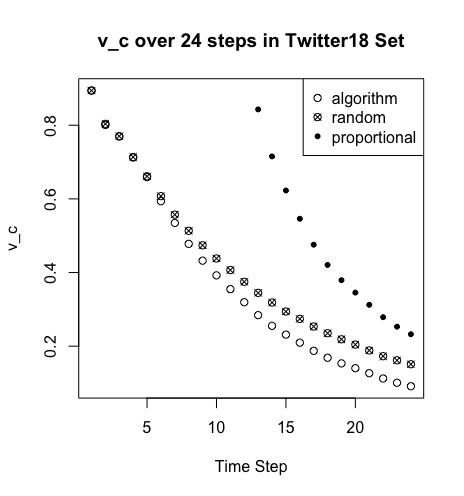
\includegraphics[width=\linewidth]{v_c in Twitter18.png}
    \caption{\textit{Twitter18} Set}
    \label{fig:mu6 Twitter18}
\endminipage\hfill
\minipage{0.32\textwidth}
  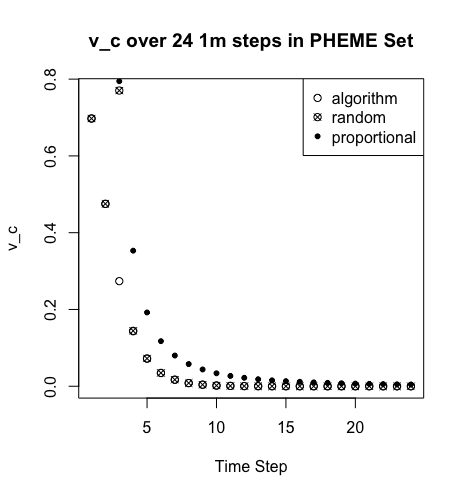
\includegraphics[width=\linewidth]{v_c PHEME 1m.png}
      \caption{\textit{PHEME}, 1m}
    \label{fig:mu6 PHEME}
\endminipage\hfill
\minipage{0.32\textwidth}
  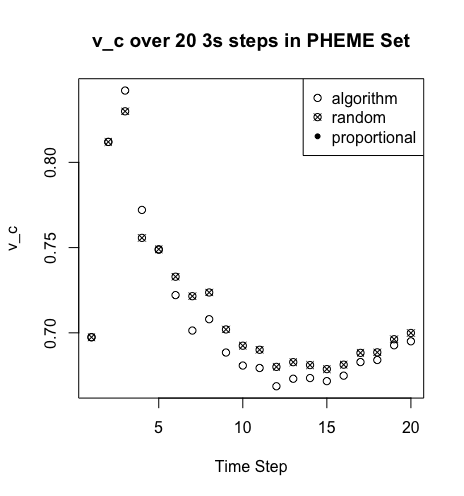
\includegraphics[width=\linewidth]{v_c pheme 3s.png}
    \caption{\textit{PHEME}, 3s}
    \label{fig:mu6 PHEME 3s}
\endminipage
\end{figure}

In this experiment, the algorithm consistently outperformed both random and proportional fact-checking. While the separation was not as high as expected, that is primarily due to the short retweet paths of the majority of the tweets being studied. All three of these data sets came with the same key caveat: they had all been batched and partitioned, meaning that each tweet path begins at time = 0. Since all of the ``super-spreader" content began at the same time, the algorithm had very few opportunities to pick between content that had been spreading rapidly, but was now stale, and new content that was showing signs of epidemic spread. The \textit{Twitter18} data set is likely the best exemplar of this: after approximately 5 time steps, the algorithm begins to show exponential improvement over both the random and proportional solutions. 

\section{Discussion, Conclusion, and Next Steps}
A reasonable person may argue that $t_2$ from the ordered set may actually be more important to fact check than $t_1$ (regardless of viral spread), as there are multiple strains of misinformation covering multiple topics every day.  For example, in late 2020, there was a wide spread in misinformation surrounding the COVID-19 vaccine \cite{mills2020covid,bagherpour2020covid}. Concurrently, false claims of fraud in the 2020 U.S. election \cite{dean2020facebook} spread before being replaced with plans for a violent insurrection on January 6th at the U.S. Capitol \cite{fandos2021trump,Levenson2021capitol}. Each of these topics is dangerous; each stands to have a high cost in human life and suffering. Reasonable people could make cogent arguments about one thread of misinformation being more or less dangerous than the other. However, fact checkers can only check so much and only check so quickly, so any ranking will leave room for criticism.

Because of that, a back-up solution would be to use this ranking system as a circuit breaker concurrently. Content where $\zeta$ is greater than a particular threshold, $\zeta_t$, can be quarantined pending fact-checking. This is not a radical proposal: circuit-breakers are used in global financial markets during times of extreme volatility \cite{wang2019microstructure,schwert1990stock} and can promote market-wide stability by ``preventing the spread of poor market quality" \cite{brugler2014single,schneider2020stock}. Indeed, this proposal has already generated discussion by experts \cite{goodman2020digital,simpson2020fighting} and Facebook has expressed interest in adding ``speed bumps" \cite{bond2020circuit}.

Regardless, this algorithm was successfully able to identify and vaccinate the super-spreaders when given the opportunity and reduced the contagiousness of the network over proportional and random fact-checking. By not attempting to catch every error and fact-check every post, the resources here are maximized. Most tweets quickly reach a dead end and have no further spread; spending any time checking them is wasted effort. As seen in figure \ref{fig:mu6 Twitter18}, after ``vaccinating" only 24 tweets from the data set, the remainder of the tweets had an extremely lower spread: at the beginning 89\% of the tweets would have to be removed to stop viral spread; at the end, only 10\% needed to be. It successfully identified the super-spreaders and targeted them first.

Finally, the resources required for this are far lower than those needed for an RNN that would attempt to check all of the 550 million tweets written per day. Many of these underlying numbers, such as $|\psi|$ values for each user, are relatively static and easily selected from the available data layers. The equations using those numbers are far less resource intensive than the perpetual training and implementation of a CNN or RNN. As mentioned in \ref{mu2}, yesterday's topics are not the same as today's topics; text/user patterns that the neural networks detected yesterday are easily changed today. That will require constant training, which will be heavily resource intensive. This algorithm solves that.

The next steps for validating this algorithm would be to use a much larger data set on computers with more sophisticated resources. Every piece of coding for this article was performed on a 2020 MacBook Air with only 8GB of RAM. Server level machines would be able to run this exact same algorithm much faster, and would be able to process the $\approx 6,366$ tweets that are posted every second on average. 

After that iteration, the next step would be to determine the $\beta$ weights for each $\mu$ value as proposed in section \ref{methodology}. While this article transformed every $\mu$ value using using minmax, after several iterations of this algorithm it may be determined that $\mu_3$ is far more important than $\mu_2$ in determining if content needs to be flagged for analysis -- the inclusion of $\beta$ weights will allow for this observation and may be re-calibrated on an iterative basis until the optimal values are discovered.

\newpage
\bibliographystyle{elsarticle-num-names} 
\bibliography{bibliography}
\end{document}


